!Programa para calcular los periodos de la marea corresponden
al manglar El Sargento
!Realizado por Inés Valenzuela

Program mareas

implicit none

 
real, dimension (7674) :: altura

integer :: i


  
real :: delta1,maxm1,maxm2,maxm3,maxm4,maxm5 !Máximos para cada mes
real ::mestx1,mestx2,mestx3,mestx4,mestx5 !Tiempo para cada máximo del mes

real :: delta2,minm1,minm2,minm3,minm4,minm5 !Mínimo para cada mes
real :: mestn1,mestn2,mestn3,mestn4,mestn5 !tiempo para cada mínimo del mes

real :: delta3,maxd1,maxd2,maxd3,maxd4,maxd5,maxd6,maxd12,maxd22,
maxd32,maxd42,maxd52,maxd62 !Máximo por cada medio día
real :: diatx1,diatx2,diatx3,diatx4,diatx5,diatx6,diatx12,diatx22,
diatx32,diatx42,diatx52,diatx62 !Tiempo de máximos por día

real :: Pm1,Pm2,Pm3,Pm4 !Período por mes
real :: Pd1,Pd2,Pd3,Pd4,Pd5,Pd6,Pd7,Pd8,Pd9,Pd10,Pd11 !Período por medio día
real :: Pm,Pd !Períodos promedio

!.......................................................................

open (1, file='mareas.csv') !Datos del nivel de la marea
open (2, file='maximosdia.dat')
open (3, file='maxmes.dat')

do i=1,7674
read (1,*) altura(i)
end do

close (1)

!........................................................................
!Encuentra el máximo para cada mes

maxm1=0
do i=1,1344
delta1=maxm1-altura(i)
if (delta1<0) then
maxm1= altura(i)
mestx1= i/48
end if
end do

WRITE (3,*) mestx1*48,maxm1

maxm2=0
do i=1345,2688
delta1=maxm2-altura(i)
if (delta1<0) then
maxm2= altura(i)
mestx2= i/48
end if
end do

WRITE (3,*) mestx2*48, maxm2 

maxm3=0
do i=2688,4032
delta1=maxm3-altura(i)
if (delta1<0) then
maxm3= altura(i)
mestx3= i/48
end if
end do

WRITE (3,*) mestx3*48, maxm3


maxm4=0
do i=4032,5376
delta1=maxm4-altura(i)
if (delta1<0) then
maxm4= altura(i)
mestx4= i/48
end if
end do

WRITE (3,*) mestx4*48, maxm4


maxm5=0
do i=5376,6720
delta1=maxm5-altura(i)
if (delta1<0) then
maxm5= altura(i)
mestx5= i/48
end if
end do

WRITE (3,*) mestx5*48, maxm5


!........................................................................
!Encuentra el mínimo para cada mes

minm1=0
do i=1,1344
delta2=minm1-altura(i)
if (delta2>0) then
minm1= altura(i)
mestn1= i/48
end if
end do

minm2=0
do i=1344,2688
delta2=minm2-altura(i)
if (delta2>0) then
minm2= altura(i)
mestn2= i/48
end if
end do

minm3=0
do i=2688,4032
delta2=minm3-altura(i)
if (delta2>0) then
minm3= altura(i)
mestn3= i/48
end if
end do

minm4=0
do i=4032,5376
delta2=minm4-altura(i)
if (delta2>0) then
minm4= altura(i)
mestn4= i/48
end if
end do

minm5=0
do i=5376,6720
delta2=minm5-altura(i)
if (delta2>0) then
minm5= altura(i)
mestn5= i/48
end if
end do

!........................................................................
!Maximos de una semana cada 12 horas

maxd1=0
do i=35,58
delta3=maxd1-altura(i)
if (delta3<0) then
maxd1=altura(i)
diatx1=i*0.5
end if
end do

WRITE (2,*) diatx1*2, maxd1 

maxd12=0
do i=59,82
delta3=maxd12-altura(i)
if (delta3<0) then
maxd12=altura(i)
diatx12=i*0.5
end if
end do

WRITE (2,*) diatx12*2,maxd12

maxd2=0
do i=83,106
delta3=maxd2-altura(i)
if (delta3<0) then
maxd2=altura(i)
diatx2=i*0.5
end if
end do

WRITE (2,*) diatx2*2,maxd2

maxd22=0
do i=107,130
delta3=maxd22-altura(i)
if (delta3<0) then
maxd22=altura(i)
diatx22=i*0.5
end if
end do

WRITE (2,*) diatx22*2,maxd22

maxd3=0
do i=131,154 
delta3=maxd3-altura(i)
if (delta3<0) then
maxd3=altura(i)
diatx3=i*0.5
end if
end do

WRITE (2,*) diatx3*2,maxd3

maxd32=0
do i=155,178
delta3=maxd32-altura(i)
if (delta3<0) then
maxd32=altura(i)
diatx32=i*0.5
end if
end do

WRITE (2,*) diatx32*2,maxd32

maxd4=0
do i=179,202
delta3=maxd4-altura(i)
if (delta3<0) then
maxd4=altura(i)
diatx4=i*0.5
end if
end do

WRITE (2,*) diatx4*2,maxd4

maxd42=0
do i=203,226
delta3=maxd42-altura(i)
if (delta3<0) then
maxd42=altura(i)
diatx42=i*0.5
end if
end do

WRITE (2,*) diatx42*2,maxd42

maxd5=0
do i=227,250
delta3=maxd5-altura(i)
if (delta3<0) then
maxd5=altura(i)
diatx5=i*0.5
end if
end do

WRITE (2,*) diatx5*2,maxd5

maxd52=0
do i=251,274
delta3=maxd52-altura(i)
if (delta3<0) then
maxd52=altura(i)
diatx52=i*0.5
end if
end do

WRITE (2,*) diatx52*2,maxd52

maxd6=0
do i=275,298
delta3=maxd6-altura(i)
if (delta3<0) then
maxd6=altura(i)
diatx6=i*0.5
end if
end do

WRITE (2,*) diatx6*2,maxd6

maxd62=0
do i=299,322
delta3=maxd62-altura(i)
if (delta3<0) then
maxd62=altura(i)
diatx62=i*0.5
end if
end do

WRITE (2,*) diatx62*2,maxd62

!........................................................................
!Períodos por mes

Pm1=(mestx2-mestx1)
Pm2=(mestx3-mestx2)
Pm3=(mestx4-mestx3)
Pm4=(mestx5-mestx4)
Pm=(pm1+pm2+pm3+pm4)/4 !Período promedio

!Períodos por día

pd1=(diatx12-diatx1)
pd2=(diatx2-diatx12)
pd3=(diatx22-diatx2)
pd4=(diatx3-diatx22)
pd5=(diatx32-diatx3)
pd6=(diatx4-diatx32)
pd7=(diatx42-diatx4)
pd8=(diatx5-diatx42)
pd9=(diatx52-diatx5)
pd10=(diatx6-diatx52)
pd11=(diatx62-diatx6)

pd =(pd1+pd2+pd3+pd4+pd5+pd6+pd7+pd8+pd9+pd10+pd11)/11 !Periodo promedio

!........................................................................


Print *,'********************************************'
Print *,'Niveles máximos de mareas mensuales:'
Print *,'............................................'
Print *,'Primer mes:', maxm1, 'El día:', mestx1
Print *,'............................................'
Print *,'Segundo mes:', maxm2, 'El día:', mestx2
Print *,'............................................'
Print *,'Tercer mes:', maxm3, 'El día:', mestx3
Print *,'............................................'
Print *,'Cuarto mes:', maxm4, 'El día:', mestx4
Print *,'............................................'
Print *,'Quinto mes:', maxm5, 'El día:', mestx5
Print *,'********************************************'
Print *,'Niveles mínimos de mareas mensuales:'
Print *,'............................................'
Print *,'Primer mes:', minm1, 'El día:', mestn1
Print *,'............................................'
Print *,'Segundo mes:', minm2, 'El día:', mestn2
Print *,'............................................'
Print *,'Tercer mes:', minm3, 'El día:', mestn3
Print *,'............................................'
Print *,'Cuarto mes:', minm4, 'El día:', mestn4
Print *,'............................................'
Print *,'Quinto mes:', minm5, 'El día:', mestn5
Print *,'********************************************'
Print *,'El período de la marea máxima por mes es:'
Print *,'............................................'
Print *,'Del primer al segundo mes:',pm1, 'días'
Print *,'............................................'
Print *,'Del segundo al tercer mes:',pm2, 'días'
Print *,'............................................'
Print *,'Del tercer al cuarto mes:',pm3,'días'
Print *,'............................................'
Print *,'Del cuarto al quinto mes:',pm4,'días'
Print *,'............................................'
Print *,'El período promedio mensual de maximos es:',Pm
Print *,'********************************************'
Print *,'Niveles máximos de mareas diarias:'
Print *,'............................................'
Print *,'Primer día:',maxd1,'y',maxd12  
Print *,'............................................'
Print *,'segundo día:',maxd2,'y',maxd22  
Print *,'............................................'
Print *,'Tercer día:',maxd3,'y',maxd32  
Print *,'............................................'
Print *,'Cuarto día:',maxd4,'y',maxd42  
Print *,'............................................'
Print *,'Quinto día:',maxd5,'y',maxd52  
Print *,'............................................'
Print *,'Sexto día:',maxd6,'y',maxd62  
Print *,'********************************************'
Print *,'El período de la marea máxima cada 12 horas:'
Print *,'............................................'
Print *,'del primer día :',pd1
Print *,'............................................'
Print *,'del primer al segundo día :',pd2
Print *,'............................................'
Print *,'del segundo día :',pd3
Print *,'............................................'
Print *,'del segundo al tercer día :',pd4
Print *,'............................................'
Print *,'del tercer día :',pd5
Print *,'............................................'
Print *,'del tercer al cuarto día :',pd6
Print *,'............................................'
Print *,'del cuarto día :',pd7
Print *,'............................................'
Print *,'del cuarto al quinto día :',pd8
Print *,'............................................'
Print *,'del quinto día :',pd9
Print *,'............................................'
Print *,'del quinto al sexto día :',pd10
Print *,'............................................'
Print *,'del sexto día :',pd11
Print *,'............................................'
Print *,'El período promedio diario de maximos es:',Pd


end program mareas


\end{verbatim}

\subsection{Resultados}

El programa arrojó los siguientes resultados:

\begin{figure}[ht]
\centering
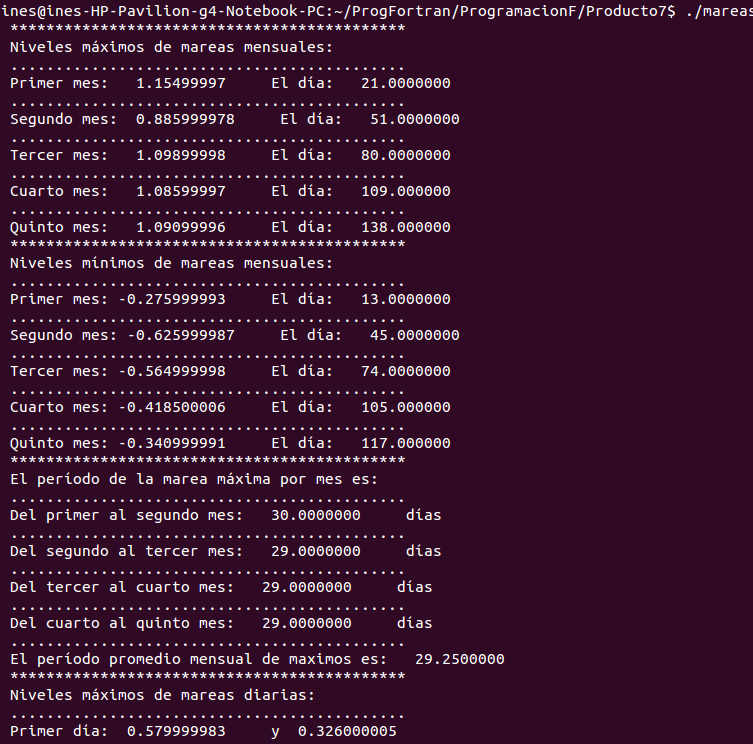
\includegraphics[width=10 cm]{terminal1.png}
\end{figure}

\begin{figure}[ht]
\centering
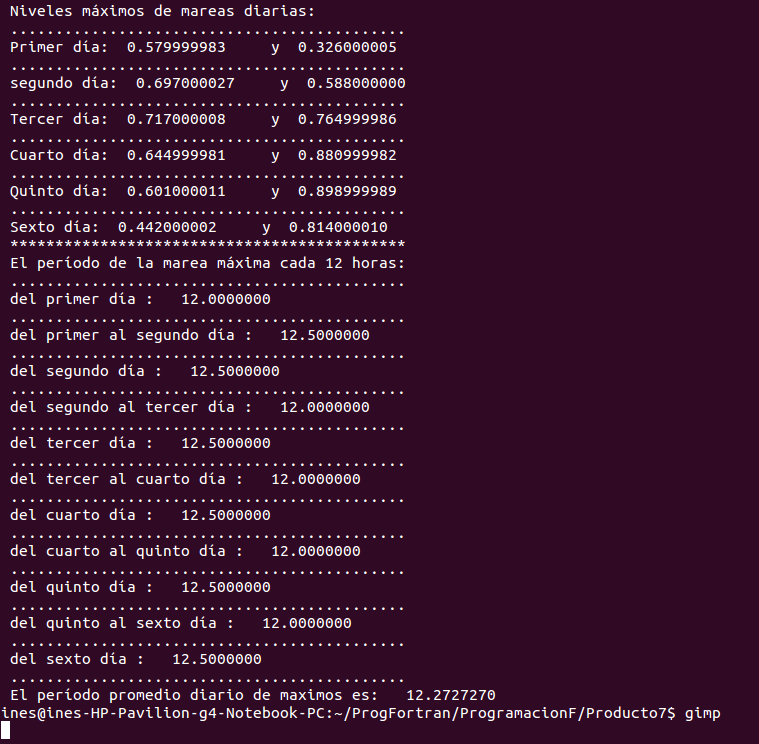
\includegraphics[width=10 cm]{terminal2.png}
\end{figure}

\clearpage

\newpage 


\section{Interpretación de gráficas y resultados}

En la siguiente gráfica se pueden mostrar los registros del nivel del mar a partir de octubre hasta  marzo del siguiente año.

\begin{figure}[ht]
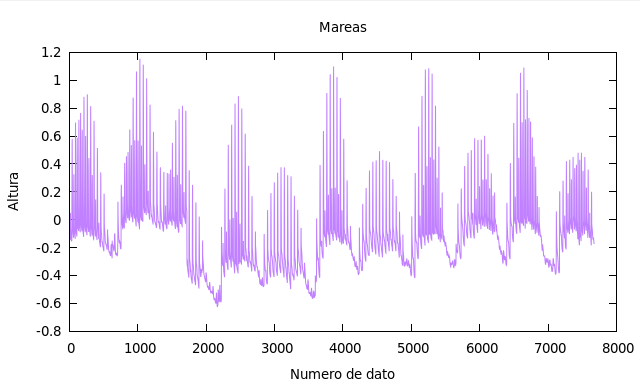
\includegraphics[width=11 cm]{mareas.png}
\end{figure}

Mediante el programa en FORTRAN obtuvimos los máximos por mes durante 5 meses y los guardamos en un archivo “maxmes.dat”.  Esta gráfica muestra el contraste entre los datos que nos proporcionaron inicialmente y los máximos que se encontraron por mes. Como se puede ver en la gráfica los puntos máximos coinciden y se tiene solamente uno en el mes, lo cual es lógico debido a que el periodo encontrado fue de aproximadamente 29 días, es decir, el pleamar máximo de cada mes ocurre en ese lapso de tiempo.



\begin{figure}[ht]
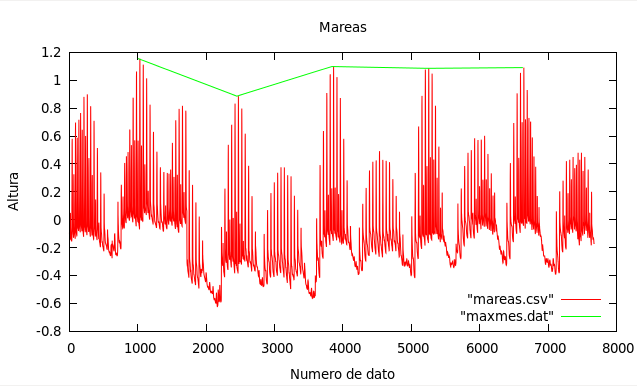
\includegraphics[width=11 cm]{maxmes.png}
\end{figure}

Por último, la gráfica que a continuación se muestra señala los máximos durante 6 días del mes de octubre, al igual que en la anterior se compara con los datos que nos dieron inicialmente, pero esta vez en un rango más pequeño. 

Todos los máximos coinciden, y los resultados del programa nos  indican que el periodo entre cada pleamar es de aproximadamente 12 horas, por lo tanto es fácil concluir que se tienen dos máximos por día. Con lo anterior se puede deducir que no es una marea diurna, en donde se tiene solo un pleamar por día, sino que es una semi-diurna ya que cuenta con dos pleamar y dos bajamar cada día. 

\begin{figure}[ht]
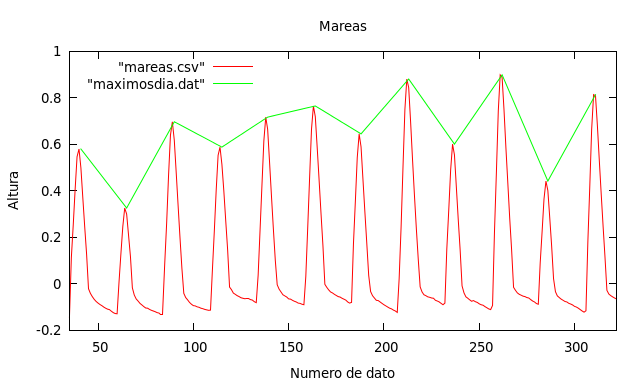
\includegraphics[width=11 cm]{maxdia.png}
\end{figure}

\end{document}
